\documentclass[fleqn,9pt,t]{beamer}

\usepackage[english]{babel}
\usepackage[utf8]{inputenc}
\usepackage[T1]{fontenc}
%\usepackage{french} % Sommaire en début de document
%\usepackage[top=2cm, bottom=2cm, left=2cm, right=2cm]{geometry} % Marges

\usepackage{amsmath} % Maths
\usepackage{amsfonts} % Maths
\usepackage{amssymb} % Maths
\usepackage{stmaryrd} % Maths (crochets doubles)

%\usepackage{listings} % Mise en forme du code (pour Hoare) ## À REVOIR ###
%\usepackage{ifthen} % Structures If Then Else
\usepackage{theorem} % Styles supplémentaires pour théorèmes
\usepackage{url}
\usepackage{array}  % Tableaux évolués
\usepackage{multirow}  % Pour des colonnes sur plusieurs lignes

%\usepackage{enumerate} % Changer les puces des listes d'énumération
%\usepackage{setspace} % Changer les interlignes

%\usepackage{subfig} % Créer des sous-figures
%\usepackage{graphicx} % Importer des images

\usepackage{ulem}  % Pour l'attribut barré

\usepackage{comment}

% Police
\usepackage{lmodern}
%\usepackage{libertine}


%%%%%%%%%%%%%%%%%%%%%%%%%%%%%%%%%%%%%%
\usepackage{tikz}
\newdimen\pgfex
\newdimen\pgfem
\usetikzlibrary{arrows,shapes,shadows,scopes}
\usetikzlibrary{positioning}
\usetikzlibrary{matrix}
\usetikzlibrary{decorations.text}
\usetikzlibrary{decorations.pathmorphing}

% Macros relatives à la traduction de PH avec arcs neutralisants vers PH à k-priorités fixes

% Macros générales
\newcommand{\ie}{\textit{i.e.} }

% Notations générales pour PH
\newcommand{\PH}{\mathcal{PH}}
\newcommand{\PHs}{\mathcal{S}}
%\newcommand{\PHp}{\mathcal{P}}
\newcommand{\PHp}{\textcolor{red}{\mathcal{P}}}
\newcommand{\PHproc}{\mathcal{P}}
\newcommand{\PHa}{\mathcal{A}}
\newcommand{\PHl}{\mathcal{L}}
\newcommand{\PHn}{\mathcal{N}}

\newcommand{\PHfrappeur}{\mathsf{frappeur}}
\newcommand{\PHcible}{\mathsf{cible}}
\newcommand{\PHbond}{\mathsf{bond}}
\newcommand{\PHsorte}{\mathsf{sorte}}
\newcommand{\PHbloquant}{\mathsf{bloquante}}
\newcommand{\PHbloque}{\mathsf{bloquee}}

\newcommand{\PHfrappeR}{\textcolor{red}{\rightarrow}}
\newcommand{\PHmonte}{\textcolor{red}{\Rsh}}

\newcommand{\PHfrappeA}{\rightarrow}
\newcommand{\PHfrappeB}{\Rsh}
%\newcommand{\PHfrappe}[3]{\mbox{$#1\PHfrappeA#2\PHfrappeB#3$}}
%\newcommand{\PHfrappebond}[2]{\mbox{$#1\PHfrappeB#2$}}
\newcommand{\PHfrappe}[3]{#1\PHfrappeA#2\PHfrappeB#3}
\newcommand{\PHfrappebond}[2]{#1\PHfrappeB#2}
\newcommand{\PHobjectif}[2]{\mbox{$#1\PHfrappeB^*\!#2$}}
\newcommand{\PHconcat}{::}
\newcommand{\PHneutralise}{\rtimes}

\def\PHget#1#2{{#1[#2]}}
%\newcommand{\PHchange}[2]{#1\langle #2 \rangle}
\newcommand{\PHchange}[2]{(#1 \Lleftarrow #2)}
\newcommand{\PHarcn}[2]{\mbox{$#1\PHneutralise#2$}}
\newcommand{\PHjoue}{\cdot}

\newcommand{\PHetat}[1]{\mbox{$\langle #1 \rangle$}}

% Notations spécifiques aux graphes d'états
\newcommand{\PHge}{\textcolor{red}{\mathcal{GE}}}
\newcommand{\PHt}{\mathcal{T}}
\newcommand{\GE}{\mathcal{GE}}
\newcommand{\GEt}{\mathcal{T}}
\newcommand{\GEl}{\PHl}
\newcommand{\GEa}{\PHa}
\newcommand{\GEva}[3]{#1 \stackrel{#2}{\longrightarrow} #3}
\newcommand{\GEval}[3]{#1 \stackrel{#2}{\Longrightarrow} #3}
\newcommand{\GEget}[2]{\PHget{#1}{#2}}



% Notations pour le modèle de Thomas (depuis thèse)
\def\levels{\mathsf{niveaux}}
\def\levelsA#1#2{\levels_+(#1\rightarrow #2)}
\def\levelsI#1#2{\levels_-(#1\rightarrow #2)}
\newcommand{\PHres}{\mathsf{Res}}

% Notations spécifiques au modèle de Thomas
\newcommand{\Kinconnu}{\emptyset}
\newcommand{\RRGva}[3]{#1 \stackrel{#2}{\longrightarrow} #3}
\newcommand{\RRGgi}{\mathcal{G}}
\newcommand{\RRGreg}[1]{\RRGgi_{#1}}
\newcommand{\RRGres}[2]{\PHres_{#1}(#2)}



% Notations spécifiques aux actions conjointes
\newcommand{\PHfrappeAconjointe}{\rightarrowtail}
\newcommand{\PHfrappec}[3]{\mbox{$#1\PHfrappeAconjointe#2\PHfrappeB#3$}}



% Notations spécifiques à ce document
\newcommand{\A}{}
\newcommand{\B}{'}
%\newcommand{\A}{_A}
%\newcommand{\B}{_B}
\newcommand{\simule}{\rho}
\newcommand{\relsimule}{\textcolor{red}{\lesssim}}
\newcommand{\abstraction}{\alpha}
\newcommand{\chap}[1]{\textcolor{blue}{\widehat{#1}}}

% Notations spécifiques à la traduction
\newcommand{\PHsc}{\ensuremath{sc}}
\newcommand{\PHsca}[1]{\ensuremath{\PHsc^{#1}}}
\newcommand{\PHfsc}{f_{sc}}
\newcommand{\PHjouables}{\mathsf{jouables}}

\usepackage{ifthen}
\usepackage{tikz}
\usetikzlibrary{arrows,shapes}

\definecolor{lightgray}{rgb}{0.8,0.8,0.8}
\definecolor{lightgrey}{rgb}{0.8,0.8,0.8}

\tikzstyle{boxed ph}=[]
\tikzstyle{sort}=[fill=lightgray,rounded corners]
\tikzstyle{process}=[circle,draw,minimum size=15pt,fill=white,
font=\footnotesize,inner sep=1pt]
\tikzstyle{black process}=[process, fill=black,text=white, font=\bfseries]
\tikzstyle{gray process}=[process, draw=black, fill=lightgray]
\tikzstyle{current process}=[process, draw=black, fill=lightgray]
\tikzstyle{process box}=[white,draw=black,rounded corners]
\tikzstyle{tick label}=[font=\footnotesize]
\tikzstyle{tick}=[black,-]%,densely dotted]
\tikzstyle{hit}=[->,>=angle 45]
\tikzstyle{selfhit}=[min distance=30pt,curve to]
\tikzstyle{bounce}=[densely dotted,>=stealth',->]
\tikzstyle{hl}=[font=\bfseries,very thick]
\tikzstyle{hl2}=[hl]
\tikzstyle{nohl}=[font=\normalfont,thin]

\newcommand{\currentScope}{}
\newcommand{\currentSort}{}
\newcommand{\currentSortLabel}{}
\newcommand{\currentAlign}{}
\newcommand{\currentSize}{}

\newcounter{la}
\newcommand{\TSetSortLabel}[2]{
  \expandafter\repcommand\expandafter{\csname TUserSort@#1\endcsname}{#2}
}
\newcommand{\TSort}[4]{
  \renewcommand{\currentScope}{#1}
  \renewcommand{\currentSort}{#2}
  \renewcommand{\currentSize}{#3}
  \renewcommand{\currentAlign}{#4}
  \ifcsname TUserSort@\currentSort\endcsname
    \renewcommand{\currentSortLabel}{\csname TUserSort@\currentSort\endcsname}
  \else
    \renewcommand{\currentSortLabel}{\currentSort}
  \fi
  \begin{scope}[shift={\currentScope}]
  \ifthenelse{\equal{\currentAlign}{l}}{
    \filldraw[process box] (-0.5,-0.5) rectangle (0.5,\currentSize-0.5);
    \node[sort] at (-0.2,\currentSize-0.4) {\currentSortLabel};
   }{\ifthenelse{\equal{\currentAlign}{r}}{
     \filldraw[process box] (-0.5,-0.5) rectangle (0.5,\currentSize-0.5);
     \node[sort] at (0.2,\currentSize-0.4) {\currentSortLabel};
   }{
    \filldraw[process box] (-0.5,-0.5) rectangle (\currentSize-0.5,0.5);
    \ifthenelse{\equal{\currentAlign}{t}}{
      \node[sort,anchor=east] at (-0.3,0.2) {\currentSortLabel};
    }{
      \node[sort] at (-0.6,-0.2) {\currentSortLabel};
    }
   }}
  \setcounter{la}{\currentSize}
  \addtocounter{la}{-1}
  \foreach \i in {0,...,\value{la}} {
    \TProc{\i}
  }
  \end{scope}
}

\newcommand{\TTickProc}[2]{ % pos, label
  \ifthenelse{\equal{\currentAlign}{l}}{
    \draw[tick] (-0.6,#1) -- (-0.4,#1);
    \node[tick label, anchor=east] at (-0.55,#1) {#2};
   }{\ifthenelse{\equal{\currentAlign}{r}}{
    \draw[tick] (0.6,#1) -- (0.4,#1);
    \node[tick label, anchor=west] at (0.55,#1) {#2};
   }{
    \ifthenelse{\equal{\currentAlign}{t}}{
      \draw[tick] (#1,0.6) -- (#1,0.4);
      \node[tick label, anchor=south] at (#1,0.55) {#2};
    }{
      \draw[tick] (#1,-0.6) -- (#1,-0.4);
      \node[tick label, anchor=north] at (#1,-0.55) {#2};
    }
   }}
}
\newcommand{\TSetTick}[3]{
  \expandafter\repcommand\expandafter{\csname TUserTick@#1_#2\endcsname}{#3}
}

\newcommand{\myProc}[3]{
  \ifcsname TUserTick@\currentSort_#1\endcsname
    \TTickProc{#1}{\csname TUserTick@\currentSort_#1\endcsname}
  \else
    \TTickProc{#1}{#1}
  \fi
  \ifthenelse{\equal{\currentAlign}{l}\or\equal{\currentAlign}{r}}{
    \node[#2] (\currentSort_#1) at (0,#1) {#3};
  }{
    \node[#2] (\currentSort_#1) at (#1,0) {#3};
  }
}
\newcommand{\TSetProcStyle}[2]{
  \expandafter\repcommand\expandafter{\csname TUserProcStyle@#1\endcsname}{#2}
}
\newcommand{\TProc}[1]{
  \ifcsname TUserProcStyle@\currentSort_#1\endcsname
    \myProc{#1}{\csname TUserProcStyle@\currentSort_#1\endcsname}{}
  \else
    \myProc{#1}{process}{}
  \fi
}

\newcommand{\repcommand}[2]{
  \providecommand{#1}{#2}
  \renewcommand{#1}{#2}
}
\newcommand{\THit}[5]{
  \path[hit] (#1) edge[#2] (#3#4);
  \expandafter\repcommand\expandafter{\csname TBounce@#3@#5\endcsname}{#4}
}
\newcommand{\TBounce}[4]{
  (#1\csname TBounce@#1@#3\endcsname) edge[#2] (#3#4)
}

\newcommand{\TState}[1]{
  \foreach \proc in {#1} {
    \node[current process] (\proc) at (\proc.center) {};
  }
}

% procedure, abstractions and dependencies
\newcommand{\abstr}[1]{#1^\wedge}%\text{\textasciicircum}}
\def\aBS{\abstr{\BS}}
\def\abeta{\abstr{\beta}}
\def\aZ{\abstr{\zeta}}
\def\aY{\abstr{\xi}}

\def\beforeproc{\vartriangleleft}

\def\powerset{\wp}

\def\Sce{\mathbf{Sce}}
\def\OS{\mathbf{OS}}
\def\Obj{\mathbf{Obj}}
\def\Proc{\mathbf{Proc}}

\usepackage{galois}
\newcommand{\theOSabstr}{toOS}
\newcommand{\OSabstr}[1]{\theOSabstr(#1)}
\newcommand{\theOSconcr}{toSce}
\newcommand{\OSconcr}[1]{\theOSconcr(#1)}

% \def\gO{\mathbb{O}}
% \def\gS{\mathbb{S}}
\def\aS{\mathcal{A}}
\def\Req{\mathrm{Req}}
\def\Sol{\mathrm{Sol}}
\def\Cont{\mathrm{Cont}}
\def\cBS{\BS_\ctx}
\def\caBS{\aBS_\ctx}
\def\caS{\aS_\ctx}
\def\cSol{\Sol_\ctx}
\def\cReq{\Req_\ctx}
\def\cCont{\Cont_\ctx}

\def\any{\star}

% \def\gProc{\mathrm{maxPROC}}
\def\mCtx{\mathrm{maxCtx}}

\def\procs{\f{procs}}
\def\objs{\f{objs}}
\def\sat#1{\lceil #1\rceil}

\def\gCont{\f{maxCont}}
\def\lCont{\f{minCont}}
\def\lProc{\f{minProc}}
\def\gProc{\f{maxProc}}

\def\join{\oplus}
\def\concat{\!::\!}
\def\ltw{\preccurlyeq_{\OS}}
\def\indexes#1{\mathbb{I}^{#1}}
%\def\indexes#1{\{1..|#1|\}}
\def\supp{\f{support}}
\def\w{\omega}
\def\W{\Omega}
\def\ctx{\varsigma}
\def\Ctx{\mathbf{Ctx}}
\def\mconcr{\gamma}
\def\concr{\mconcr_\ctx}
\def\obj#1#2{{#1\!\Rsh^*\!\!#2}}
\def\objp#1#2#3{\obj{{#1}_{#2}}{{#1}_{#3}}}
\def\A{\mathcal{A}}
\def\cwA{\A_\ctx^\w}
\def\cwReq{\Req_\ctx^\w}
\def\cwSol{\Sol_\ctx^\w}
\def\cwCont{\Cont_\ctx^\w}
\def\gCtx{\f{maxCtx}}
\def\endCtx{\f{endCtx}}
\def\ceil{\f{end}}

\def\lfp{\mathrm{lfp}\;}
\def\mlfp#1{\mathrm{lfp}\{#1\}\;}
\def\maxobjs{{\f{maxobjs}}}
\def\maxprocs{{\f{maxprocs}_\ctx}}
\def\objends{{\f{ends}}}

\def\ra{\rho}
\def\rb{\rho^\wedge}
\def\rc{\widetilde{\rho}}
\def\interleave{\f{interleave}}

\def\join{\concat}

\def\Pint{\textsc{PINT}}
\def\PH{\mathcal{PH}}

\tikzstyle{sort}=[fill=lightgray, rounded corners, draw=black]
\tikzstyle{process}=[circle,draw,minimum size=15pt,font=\footnotesize,inner sep=1pt]
\tikzstyle{black process}=[process, draw=blue, fill=red,text=black,font=\bfseries]
\tikzstyle{highlighted process}=[current process, fill=gray]
\tikzstyle{process box}=[fill=none,draw=black,rounded corners]
\tikzstyle{current process}=[process,fill=blue]
\tikzstyle{tick label}=[font=\footnotesize]
\tikzstyle{tick}=[densely dotted]
\tikzstyle{hit}=[->,>=angle 45]
\tikzstyle{selfhit}=[min distance=30pt,curve to]
\tikzstyle{bounce}=[densely dotted,>=stealth',->]
\tikzstyle{hlhit}=[very thick]
\tikzstyle{ulhit}=[draw=lightgray,fill=lightgray]
\tikzstyle{pulhit}=[fill=lightgray]
\tikzstyle{bulhit}=[draw=lightgray]

\tikzstyle{hitless graph}=[every edge/.style={draw=red,-}]

\tikzstyle{aS}=[every edge/.style={draw,->}]
\tikzstyle{Asol}=[draw,circle,minimum size=5pt,inner sep=0]
\tikzstyle{Aproc}=[draw]
\tikzstyle{Aobj}=[]

\renewcommand{\TState}[2]{
  \foreach \proc in {#2} {
        \only<#1>{ \node[current process] (\proc) at (\proc.center) {}; }
  };
}

%\definecolor{darkred}{rgb}{0.5,0,0}
\definecolor{lightred}{rgb}{1,0.8,0.8}
\definecolor{lightgreen}{rgb}{0.7,1,0.7}
\definecolor{darkgreen}{rgb}{0,0.5,0}
\definecolor{darkblue}{rgb}{0,0,0.5}
\definecolor{darkyellow}{rgb}{0.5,0.5,0}
\definecolor{lightyellow}{rgb}{1,1,0.6}
\definecolor{darkcyan}{rgb}{0,0.6,0.6}
\definecolor{darkorange}{rgb}{0.8,0.2,0}

\definecolor{notsodarkgreen}{rgb}{0,0.7,0}

%\definecolor{coloract}{rgb}{0,1,0}
%\definecolor{colorinh}{rgb}{1,0,0}
\colorlet{coloract}{darkgreen}
\colorlet{colorinh}{red}
\colorlet{coloractgray}{lightgreen}
\colorlet{colorinhgray}{lightred}
\colorlet{colorinf}{darkgray}
\colorlet{coloractgray}{lightgreen}
\colorlet{colorinhgray}{lightred}

\colorlet{colorgray}{lightgray}


\tikzstyle{grn}=[every node/.style={circle,draw=black,outer sep=2pt,minimum
                size=15pt,text=black}, node distance=1.5cm]
\tikzstyle{inh}=[>=|,-|,draw=colorinh,thick, text=black,label]
\tikzstyle{act}=[->,>=triangle 60,draw=coloract,thick,color=coloract]
\tikzstyle{inhgray}=[>=|,-|,draw=colorinhgray,thick, text=black,label]
\tikzstyle{actgray}=[->,>=triangle 60,draw=coloractgray,thick,color=coloractgray]
\tikzstyle{inf}=[->,draw=colorinf,thick,color=colorinf]
%\tikzstyle{elabel}=[fill=none, above=-1pt, sloped,text=black, minimum size=10pt, outer sep=0, font=\scriptsize,draw=none]
\tikzstyle{elabel}=[fill=none,text=black, above=-2pt,%sloped,
minimum size=10pt, outer sep=0, font=\scriptsize, draw=none]
%\tikzstyle{elabel}=[]


\tikzstyle{plot}=[every path/.style={-}]
\tikzstyle{axe}=[gray,->,>=stealth']
\tikzstyle{ticks}=[font=\scriptsize,every node/.style={gray}]
\tikzstyle{mean}=[thick]
\tikzstyle{interval}=[line width=5pt,red,draw opacity=0.7]
\definecolor{lightred}{rgb}{1,0.3,0.3}

\tikzstyle{hl}=[yellow]
\tikzstyle{hl2}=[orange]

\tikzstyle{every matrix}=[ampersand replacement=\&]
\tikzstyle{shorthandoff}=[]
\tikzstyle{shorthandon}=[]
%%%%%%%%%%%%%%%%%%%%%%%%%%%%%%%%%%%%%%%%



% Commande À FAIRE
\usepackage{color} % Couleurs du texte
\newcommand{\afaire}[1]{\textcolor{red}{[À FAIRE : #1]}}
\newcommand{\todo}[1]{\textcolor{darkgreen}{[\textcolor{red}{#1}]}}



\colorlet{couleurtheme}{gray}  % Couleur principale du thème
\colorlet{couleurcit}{gray}  % Couleur des citations
\colorlet{couleurex}{blue}  % Couleur des citations
\colorlet{couleurliens}{darkblue}  % Couleur des citations

\usetheme{Pittsburgh}   % Thème général
\usefonttheme{default}  % Thème de polices
\setbeamertemplate{navigation symbols}{}  % Pas de menu de navigation
%\setbeamertemplate{itemize item}[x]   % Puces des listes

\usecolortheme[named=couleurtheme]{structure}    % Couleur de la structure : titres et puces
%\setbeamercolor{normal text}{bg=black,fg=white}  % Couleur du texte
\setbeamercolor{item}{fg=couleurtheme}           % Couleur des puces
%\setbeamercolor{item projected}{fg=black}        % Couleur des recouvrements
%\setbeamercolor{alerted text}{fg=yellow}         % ?

\setbeamerfont{frametitle}{size=\Large}  % Police des titres


% Flèche grise
\newcommand{\f}{\textcolor{couleurtheme}{\textbf{$\rightarrow$\ }}}

% Environnement liste avec flèches
\newenvironment{fleches}{%
\begin{list}{}{%
\setlength{\labelwidth}{1em}% largeur de la boîte englobant le label
\setlength{\labelsep}{0pt}% espace entre paragraphe et l’étiquette
%\setlength{\itemsep}{1pt}
%\setlength{\leftmargin}{\labelwidth+\labelsep}% marge de gauche
\renewcommand{\makelabel}{\f}%
}}{\end{list}}

% Liste sans puce
\newenvironment{liste}{%
\begin{list}{}{%
\setlength{\labelwidth}{0em}% largeur de la boîte englobant le label
\setlength{\labelsep}{0pt}% espace entre paragraphe et l’étiquette
\setlength{\leftmargin}{0em}% marge de gauche
%\renewcommand{\makelabel}{\f}%
}}{\end{list}}

% Style des exemples
\newcommand{\ex}[1]{\textcolor{couleurex}{#1}}
\newcommand{\qex}[1]{\quad \ex{#1}}
\newcommand{\rex}[1]{\hfill \ex{#1}}

\newcommand{\lien}[1]{\textcolor{couleurliens}{\texttt{\underline{\ex{#1}}}}}

\newcommand{\console}[1]{\textcolor{darkgray}{#1}}

% Style des citations
\newcommand{\tscite}[1]{\textcolor{couleurcit}{#1}}
\newcommand{\tcite}[1]{\textcolor{couleurcit}{[#1]}}

% Style de texte mis en valeur
\newcommand{\tval}[1]{\textbf{#1}}

% Un vrai symbole pour l'ensemble vide
\renewcommand{\emptyset}{\varnothing}

% Pour définir la conférence et son nom court
\newcommand{\conference}[2]{\def\theconference{#2}
\def\insertshortconference{\ifthenelse{\equal{#1}{-}}{#2}{\ifthenelse{\equal{#1}{}}{#2}{#1}}}}



\newcommand{\thedate}{2012/10/04}
\date{\thedate}
\conference{CMSB'2012}{--- CMSB'2012 ---\\The 10\textsuperscript{th} Conference on Computational Methods in Systems Biology}
\title[Concretizing the PH into BRNs]{Concretizing the Process Hitting\\into Biological Regulatory Networks}
\author{Maxime FOLSCHETTE}




\setbeamertemplate{footline}{\color{gray}%
\scriptsize
\quad\strut%
\insertauthor%
\hfill%
\insertframenumber/\inserttotalframenumber%
\hfill%
\insertshortconference{} --- \thedate\quad\strut
}


\newcommand{\headersep}{$\circ$} % \bullet \triangleright

\setbeamertemplate{headline}{\color{gray}%
\vskip0.3em%
\quad\strut%
{\scriptsize\color{black}%
% Gris si une section existe
\ifthenelse{\equal{\thesection}{0}}{}{%
\ifthenelse{\equal{\lastsection}{x}}{}{%
\color{gray}%
}}%
\insertshorttitle
\ifthenelse{\equal{\thesection}{0}}{}{%
\ifthenelse{\equal{\lastsection}{x}}{}{%
~\headersep{} %
% Gris si une sous-section existe
\ifthenelse{\equal{\thesubsection}{0}}{\color{black}}{%
\ifthenelse{\equal{\lastsubsection}{x}}{\color{black}}{%
\color{gray}%
}}%
\insertsectionhead%
%
\ifthenelse{\equal{\thesubsection}{0}}{}{%
\ifthenelse{\equal{\lastsubsection}{x}}{}{%
~\headersep{} \color{black}\insertsubsectionhead%
%
}}}}}%
\vskip-5ex%
}



\def \scaleex {0.85}
\def \scaleinf {0.6}

\colorlet{colorb}{darkgray}
\colorlet{colora1}{yellow}
\colorlet{colora0}{green}
\colorlet{colora1font}{darkyellow}
\colorlet{colora0font}{darkgreen}

\colorlet{exanswer}{blue}
\colorlet{colorgray}{lightgray}

\definecolor{colortitle}{rgb}{0.54,0.8,0.9}


\begin{document}

\begin{frame}[plain,label=title]

% Cadre de titre
\begin{center}
\vspace{0.5cm}
\setbeamercolor{postit}{fg=black,bg=colortitle}
\begin{beamercolorbox}[sep=0.5em]{postit}
\centering
\Large
\textbf{%
{\normalsize\theconference{}}\\~\\%
\inserttitle
}
\end{beamercolorbox}

% Auteurs et instituts
\par
\medskip
\normalsize
Maxime FOLSCHETTE$^{1,2}$
\footnotesize

\texttt{maxime.folschette@irccyn.ec-nantes.fr}

\url{http://www.irccyn.ec-nantes.fr/~folschet/}

\normalsize
\bigskip
\tval{Joint work with:} Loïc PAULEVÉ$^3$, \\ Katsumi INOUE$^2$, Morgan MAGNIN$^1$, Olivier ROUX$^1$

\medskip
\footnotesize
$^1$ MeForBio / IRCCyN / École Centrale de Nantes (Nantes, France)

\texttt{morgan.magnin@irccyn.ec-nantes.fr}

\texttt{olivier.roux@irccyn.ec-nantes.fr}

\medskip
$^2$ Inoue Laboratory / NII / Sokendai University (Tokyo, Japan)

\texttt{ki@nii.ac.jp}

\medskip
$^3$ AMIB / LIX / École Polytechnique (Palaiseau, France)

\texttt{pauleve@lix.polytechnique.fr}

\bigskip
\normalsize
AtlanSTIC sojourn financed by NII \& Centrale Initiatives
\end{center}


\end{frame}


% Exemples

%%% Exemple pour la définition du Process Hitting %%%
\def \exphdef {
\path[use as bounding box] (-0.5,-0.5) rectangle (6.5,4.5);

\TSort{(0,3)}{a}{2}{l}
\TSort{(0,0)}{b}{2}{l}
\TSort{(6,1)}{z}{3}{r}

\THit{a_1}{}{z_1}{.west}{z_2}
\THit{b_1}{}{z_0}{.west}{z_1}
\THit{a_0}{out=250,in=200,selfhit}{a_0}{.west}{a_1}

\path[bounce,bend left]
\TBounce{z_0}{}{z_1}{.south}
\TBounce{z_1}{}{z_2}{.south}
\TBounce{a_0}{}{a_1}{.south}
;
}



%%% Exemple pour la coopération %%%
\def \exphcoop {
\path[use as bounding box] (-0.5,-0.5) rectangle (6.5,4.5);

% Actions de màj grisées
\only<6->{
\THit{a_1}{ulhit,color=lightgray}{ab_0}{.west}{ab_2}
\THit{a_1}{ulhit,color=lightgray}{ab_1}{.west}{ab_3}
\path[bounce,bend left,pulhit] \TBounce{ab_0}{bulhit}{ab_2}{.south} \TBounce{ab_1}{bulhit}{ab_3}{.south} ;
}

\only<7->{
\THit{a_0}{ulhit}{ab_2}{.west}{ab_0}
\THit{a_0}{ulhit}{ab_3}{.west}{ab_1}
\path[bounce,bend right,pulhit] \TBounce{ab_2}{bulhit}{ab_0}{.north} \TBounce{ab_3}{bulhit}{ab_1}{.north} ;
}

\only<8->{
\THit{b_0}{ulhit}{ab_3}{.west}{ab_2}
\THit{b_0}{ulhit}{ab_1}{.west}{ab_0}
\THit{b_1}{ulhit}{ab_0}{.west}{ab_1}
\THit{b_1}{ulhit}{ab_2}{.west}{ab_3}
\path[bounce,bend right,pulhit] \TBounce{ab_1}{bulhit}{ab_0}{.north} \TBounce{ab_3}{bulhit}{ab_2}{.north} ;
\path[bounce,bend left,pulhit] \TBounce{ab_0}{bulhit}{ab_1}{.south} \TBounce{ab_2}{bulhit}{ab_3}{.south} ;
}

% Sortes
\TSort{(0,3)}{a}{2}{l}
\TSort{(0,0)}{b}{2}{l}
\TSort{(6,1)}{z}{3}{r}

% Deux actions disjointes en exemple
\only<2-3>{
\THit{a_1}{}{z_1}{.north west}{z_2}
\path[bounce,bend left]
\TBounce{z_1}{}{z_2}{.south} ;

\THit{b_0}{}{z_1}{.west}{z_2}
\path[bounce,bend left=55]
\TBounce{z_1}{}{z_2}{.south west} ;
}

% Processus d'exemple
\TState{3}{a_1,b_1,z_1}

% Sorte coopérative et arcs
\only<4->{
\TSetTick{ab}{0}{00}
\TSetTick{ab}{1}{01}
\TSetTick{ab}{2}{10}
\TSetTick{ab}{3}{11}
\TSort{(3,0.5)}{ab}{4}{l}
}

% Arcs de màj noirs de la sc
\only<5>{
\THit{a_1}{thick}{ab_0}{.west}{ab_2}
\THit{a_1}{thick}{ab_1}{.west}{ab_3}
\path[bounce,thick,bend left] \TBounce{ab_0}{thick}{ab_2}{.south} \TBounce{ab_1}{thick}{ab_3}{.south} ;
}

\only<6>{
\THit{a_0}{thick}{ab_2}{.west}{ab_0}
\THit{a_0}{thick}{ab_3}{.west}{ab_1}
\path[bounce,thick,bend right] \TBounce{ab_2}{thick}{ab_0}{.north} \TBounce{ab_3}{thick}{ab_1}{.north} ;
}

\only<7>{
\THit{b_0}{thick}{ab_3}{.west}{ab_2}
\THit{b_0}{thick}{ab_1}{.west}{ab_0}
\THit{b_1}{thick}{ab_0}{.west}{ab_1}
\THit{b_1}{thick}{ab_2}{.west}{ab_3}
\path[bounce,thick,bend right] \TBounce{ab_1}{thick}{ab_0}{.north} \TBounce{ab_3}{thick}{ab_2}{.north} ;
\path[bounce,thick,bend left] \TBounce{ab_0}{thick}{ab_1}{.south} \TBounce{ab_2}{thick}{ab_3}{.south} ;
}

% État d'exemple pour màj de la sc
\TState{8-9}{a_1,b_0}
\TState{10}{a_1,b_0,ab_0,ab_1,ab_2,ab_3}
\TState{11}{a_1,b_0,ab_2}
\only<9-11>{
\THit{a_1}{}{ab_0}{.west}{ab_2}
\THit{a_1}{}{ab_1}{.west}{ab_3}
\THit{b_0}{}{ab_3}{.west}{ab_2}
\THit{b_0}{}{ab_1}{.west}{ab_0}
\path[bounce,bend left] \TBounce{ab_0}{}{ab_2}{.south} \TBounce{ab_1}{}{ab_3}{.south} ;
\path[bounce,bend right] \TBounce{ab_1}{}{ab_0}{.north} \TBounce{ab_3}{}{ab_2}{.north} ;
}

% État d'exemple pour action de la sc
\TState{12}{a_1,b_0,z_1,ab_2}
\TState{13-14}{a_1,b_0,z_2,ab_2}

% Arc sortant de la sc
\only<12-14>{
\THit{ab_2}{thick}{z_1}{.west}{z_2}
\path[bounce,bend left,thick] \TBounce{z_1}{thick}{z_2}{.south} ;
}

% Arc sortant de la sc
\only<15->{
\THit{ab_2}{}{z_1}{.west}{z_2}
\path[bounce,bend left] \TBounce{z_1}{}{z_2}{.south} ;
}

}



%%% Exemple pour l'inférence %%%
\def \exphinf {
% Sortes
\TSort{(0,3)}{a}{2}{l}
\TSort{(0,0)}{b}{2}{l}
\TSort{(6,0)}{z}{3}{r}

% Sorte coopérative et arcs
\TSetTick{ab}{0}{00}
\TSetTick{ab}{1}{01}
\TSetTick{ab}{2}{10}
\TSetTick{ab}{3}{11}
\TSort{(3,0)}{ab}{4}{l}

% Actions de màj grisées
\THit{a_1}{ulhit}{ab_0}{.west}{ab_2}
\THit{a_1}{ulhit}{ab_1}{.west}{ab_3}
\path[bounce,bend left,pulhit] \TBounce{ab_0}{bulhit}{ab_2}{.south} \TBounce{ab_1}{bulhit}{ab_3}{.south};

\THit{a_0}{ulhit}{ab_2}{.west}{ab_0}
\THit{a_0}{ulhit}{ab_3}{.west}{ab_1}
\path[bounce,bend right,pulhit] \TBounce{ab_2}{bulhit}{ab_0}{.north} \TBounce{ab_3}{bulhit}{ab_1}{.north};

\THit{b_0}{ulhit}{ab_3}{.west}{ab_2}
\THit{b_0}{ulhit}{ab_1}{.west}{ab_0}
\THit{b_1}{ulhit}{ab_0}{.west}{ab_1}
\THit{b_1}{ulhit}{ab_2}{.west}{ab_3}
\path[bounce,bend right,pulhit] \TBounce{ab_1}{bulhit}{ab_0}{.north} \TBounce{ab_3}{bulhit}{ab_2}{.north};
\path[bounce,bend left,pulhit] \TBounce{ab_0}{bulhit}{ab_1}{.south} \TBounce{ab_2}{bulhit}{ab_3}{.south};

% Arcs sortant de la sc
\THit{ab_2}{ulhit}{z_1}{.north west}{z_2}
\THit{ab_2}{ulhit}{z_0}{.west}{z_1}
\path[bounce,bend left,pulhit] \TBounce{z_1}{bulhit}{z_2}{.south} \TBounce{z_0}{bulhit}{z_1}{.south};

\THit{ab_3}{ulhit}{z_2}{.west}{z_1}
\THit{ab_3}{ulhit}{z_0}{.west}{z_1}
\THit{ab_1}{ulhit}{z_2}{.west}{z_1}
\THit{ab_1}{ulhit}{z_0}{.west}{z_1}
\path[bounce,bend left,pulhit] \TBounce{z_2}{bulhit,bend right}{z_1}{.north};

\THit{ab_0}{ulhit}{z_2}{.west}{z_1}
\THit{ab_0}{ulhit}{z_1}{.south west}{z_0}
\path[bounce,bend right,pulhit] \TBounce{z_2}{bulhit}{z_1}{.north} \TBounce{z_1}{bulhit}{z_0}{.north};

}



%%% Exemple pour l'inférence (sans arcs grisés) %%%
\def \exphinfblack {
% Sortes
\TSort{(0,3)}{a}{2}{l}
\TSort{(0,0)}{b}{2}{l}
\TSort{(6,0)}{z}{3}{r}

% Sorte coopérative et arcs
\TSetTick{ab}{0}{00}
\TSetTick{ab}{1}{01}
\TSetTick{ab}{2}{10}
\TSetTick{ab}{3}{11}
\TSort{(3,0)}{ab}{4}{l}

% Actions de màj grisées
\THit{a_1}{}{ab_0}{.west}{ab_2}
\THit{a_1}{}{ab_1}{.west}{ab_3}
\path[bounce,bend left] \TBounce{ab_0}{}{ab_2}{.south} \TBounce{ab_1}{}{ab_3}{.south};

\THit{a_0}{}{ab_2}{.west}{ab_0}
\THit{a_0}{}{ab_3}{.west}{ab_1}
\path[bounce,bend right] \TBounce{ab_2}{}{ab_0}{.north} \TBounce{ab_3}{}{ab_1}{.north};

\THit{b_0}{}{ab_3}{.west}{ab_2}
\THit{b_0}{}{ab_1}{.west}{ab_0}
\THit{b_1}{}{ab_0}{.west}{ab_1}
\THit{b_1}{}{ab_2}{.west}{ab_3}
\path[bounce,bend right] \TBounce{ab_1}{}{ab_0}{.north} \TBounce{ab_3}{}{ab_2}{.north};
\path[bounce,bend left] \TBounce{ab_0}{}{ab_1}{.south} \TBounce{ab_2}{}{ab_3}{.south};

% Arcs sortant de la sc
\THit{ab_2}{}{z_1}{.north west}{z_2}
\THit{ab_2}{}{z_0}{.west}{z_1}
\path[bounce,bend left] \TBounce{z_1}{}{z_2}{.south} \TBounce{z_0}{}{z_1}{.south};

\THit{ab_3}{}{z_2}{.west}{z_1}
\THit{ab_3}{}{z_0}{.west}{z_1}
\THit{ab_1}{}{z_2}{.west}{z_1}
\THit{ab_1}{}{z_0}{.west}{z_1}
\path[bounce,bend left] \TBounce{z_2}{,bend right}{z_1}{.north};

\THit{ab_0}{}{z_2}{.west}{z_1}
\THit{ab_0}{}{z_1}{.south west}{z_0}
\path[bounce,bend right] \TBounce{z_2}{}{z_1}{.north} \TBounce{z_1}{}{z_0}{.north};

}



%%% Exemple 2 pour l'inférence (projections) %%%
\def \exphinfproj {
% Sortes
\TSort{(0,3)}{a}{2}{l}
\TSort{(0,0)}{b}{2}{l}
\TSort{(6,1)}{z}{2}{r}

% Sorte coopérative et arcs
\TSetTick{ab}{0}{00}
\TSetTick{ab}{1}{01}
\TSetTick{ab}{2}{10}
\TSetTick{ab}{3}{11}
\TSort{(3,0)}{ab}{4}{l}

% Actions de màj grisées
\THit{a_1}{ulhit}{ab_0}{.west}{ab_2}
\THit{a_1}{ulhit}{ab_1}{.west}{ab_3}
\path[bounce,bend left,pulhit] \TBounce{ab_0}{bulhit}{ab_2}{.south} \TBounce{ab_1}{bulhit}{ab_3}{.south} ;

\THit{a_0}{ulhit}{ab_2}{.west}{ab_0}
\THit{a_0}{ulhit}{ab_3}{.west}{ab_1}
\path[bounce,bend right,pulhit] \TBounce{ab_2}{bulhit}{ab_0}{.north} \TBounce{ab_3}{bulhit}{ab_1}{.north} ;

\THit{b_0}{ulhit}{ab_3}{.west}{ab_2}
\THit{b_0}{ulhit}{ab_1}{.west}{ab_0}
\THit{b_1}{ulhit}{ab_0}{.west}{ab_1}
\THit{b_1}{ulhit}{ab_2}{.west}{ab_3}
\path[bounce,bend right,pulhit] \TBounce{ab_1}{bulhit}{ab_0}{.north} \TBounce{ab_3}{bulhit}{ab_2}{.north} ;
\path[bounce,bend left,pulhit] \TBounce{ab_0}{bulhit}{ab_1}{.south} \TBounce{ab_2}{bulhit}{ab_3}{.south} ;

% Arcs sortant de la sc
\THit{ab_3}{ulhit}{z_0}{.west}{z_1}
\path[bounce,bend left,pulhit] \TBounce{z_0}{bulhit}{z_1}{.south} ;

\THit{ab_0}{ulhit}{z_1}{.west}{z_0}
\path[bounce,bend right,pulhit]\TBounce{z_1}{bulhit}{z_0}{.north} ;
}



%%% Exemple sans sorte coopérative pour l'inférence %%%
\def \exphinfprojssc {
% Sortes
\TSort{(0,3)}{a}{2}{l}
\TSort{(0,0)}{b}{2}{l}
\TSort{(6,0)}{z}{3}{r}

\THit{a_1}{ulhit}{z_0}{.west}{z_1}
\THit{a_1}{ulhit}{z_1}{.north west}{z_2}
\THit{a_0}{ulhit}{z_1}{.south west}{z_0}
\THit{a_0}{ulhit}{z_2}{.west}{z_1}
\path[bounce,bend left,pulhit] \TBounce{z_0}{bulhit}{z_1}{.south} \TBounce{z_1}{bulhit}{z_2}{.south}
  \TBounce{z_1}{bulhit,bend right}{z_0}{.north} \TBounce{z_2}{bulhit,bend right}{z_1}{.north} ;

\THit{b_0}{ulhit}{z_0}{.west}{z_1}
\THit{b_0}{ulhit}{z_1}{.north west}{z_2}
\THit{b_1}{ulhit}{z_1}{.south west}{z_0}
\THit{b_1}{ulhit}{z_2}{.west}{z_1}
%\path[bounce,bend left,pulhit] \TBounce{z_0}{bulhit}{z_1}{.south} \TBounce{z_1}{bulhit}{z_2}{.south}
%  \TBounce{z_1}{bulhit,bend right}{z_0}{.north} \TBounce{z_2}{bulhit,bend right}{z_1}{.north} ;
}


\section{Introduction}
% Diapo d'intro

\begin{frame}[c]
  \frametitle{Context and Aims}

Algebraic modeling to study complex dynamical biological systems:

%\bigskip
\begin{center}
  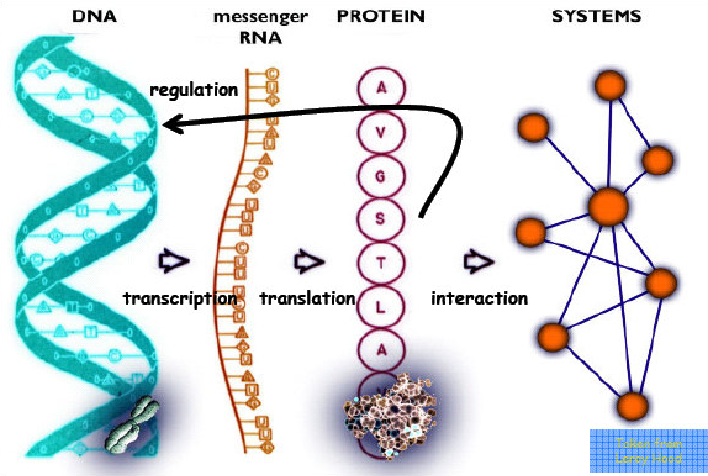
\includegraphics[height=3.5cm]{figs/dnascheme_white.png}
\end{center}

\pause
\begin{itemize}
  \item Historical model: Biological Regulatory Network (René Thomas)
  \item New developed model: Process Hitting
\end{itemize}

\textcolor{couleurtheme}{$\Rightarrow$} \fbox{\tval{\large Allow efficient translation from Process Hitting to BRN}} \textcolor{couleurtheme}{$\Leftarrow$}

\end{frame}


\section{Frameworks Definitions}
\subsection{The Process Hitting}
% Définition du Process Hitting + sortes coopératives

\begin{frame}
  \frametitle{The Process Hitting modeling}
  \framesubtitle{\tcite{PMR12-MSCS}}

% 1 : Sortes
\only<1>{
\tikzstyle{process}=[circle,minimum size=15pt,font=\footnotesize,inner sep=1pt]
\tikzstyle{tick label}=[color=white, font=\footnotesize]
\tikzstyle{tick}=[transparent]
\tikzstyle{hit}=[transparent]
\tikzstyle{selfhit}=[transparent, min distance=30pt,curve to]
\tikzstyle{bounce}=[transparent]
\tikzstyle{hlhit}=[transparent]
\begin{center}\scalebox{\scaleex}{
\begin{tikzpicture}
\exphdef
\end{tikzpicture}
}\end{center}
}

% 2 : Processus
\only<2>{
\tikzstyle{process}=[circle,draw,minimum size=15pt,font=\footnotesize,inner sep=1pt]
\tikzstyle{tick label}=[font=\footnotesize]
\tikzstyle{tick}=[densely dotted]
\tikzstyle{hit}=[transparent]
\tikzstyle{selfhit}=[transparent, min distance=30pt,curve to]
\tikzstyle{bounce}=[transparent]
\tikzstyle{hlhit}=[transparent]
\begin{center}\scalebox{\scaleex}{
\begin{tikzpicture}
\exphdef
\end{tikzpicture}
}\end{center}
}

% 3 : États
\only<3>{
\tikzstyle{hit}=[transparent]
\tikzstyle{selfhit}=[transparent, min distance=30pt,curve to]
\tikzstyle{bounce}=[transparent]
\tikzstyle{hlhit}=[transparent]
\begin{center}\scalebox{\scaleex}{
\begin{tikzpicture}
\exphdef

\TState{3}{a_0,b_1,z_0}
\end{tikzpicture}
}\end{center}
}

% 4 : Actions
\only<4->{
\tikzstyle{tick}=[densely dotted]
\tikzstyle{hit}=[->,>=angle 45]
\tikzstyle{selfhit}=[min distance=30pt,curve to]
\tikzstyle{bounce}=[densely dotted,>=stealth',->]
\tikzstyle{hlhit}=[very thick]
\begin{center}\scalebox{\scaleex}{
\begin{tikzpicture}
\exphdef
\TState{4}{a_0,b_1,z_0}
\TState{5}{a_0,b_1,z_1}
\TState{6}{a_1,b_1,z_1}
\TState{7}{a_1,b_1,z_2}
\end{tikzpicture}
}\end{center}
}

%\medskip
\begin{liste}
  \item \tval{Sorts}: components \qex{$a$, $b$, $z$}
\pause[2]
  \item \tval{Processes}: local states / levels of expression \qex{$z_0$, $z_1$, $z_2$}
\pause[3]
  \item \tval{States}: sets of active processes%
  \only<3-4>{\qex{$\PHetat{a_0, b_1, z_0}$}}%
  \only<5>{\qex{$\PHetat{a_0, b_1, z_1}$}}%
  \only<6>{\qex{$\PHetat{a_1, b_1, z_1}$}}%
  \only<7>{\qex{$\PHetat{a_1, b_1, z_2}$}}%
\pause[4]
  \item \tval{Actions}: dynamics \qex{\only<4>{\underline}{$\PHfrappe{b_1}{z_0}{z_1}$}, \only<4-5>{\underline}{$\PHfrappe{a_0}{a_0}{a_1}$}, \only<6>{\underline}{$\PHfrappe{a_1}{z_1}{z_2}$}}
\end{liste}
\end{frame}



\begin{frame}
  \frametitle{The Process Hitting modeling}
  \framesubtitle{\tcite{PMR12-MSCS}}

\begin{center}\scalebox{\scaleex}{
\begin{tikzpicture}
\exphcoop
\end{tikzpicture}
}\end{center}

\only<-14>{
\begin{liste}
  \item How to introduce some \tval{cooperation} between sorts? \qex{$\PHfrappe{a_1 \wedge b_0}{z_1}{z_2}$}
\pause[4]
  \item Solution: a \tval{cooperative sort} \qex{$ab$} \only<12->{\quad to express \qex{$a_1 \wedge b_0$}}
\pause[8]
  \item Constraint: each configuration is represented by one process \qex{$\PHetat{a_1,b_0} \pause[11]\Rightarrow ab_{10}$}
\pause[14]
  \item Advantage: regular sort; drawbacks: complexity, temporal shift
\end{liste}
}

\only<15->{
The Process Hitting framework:

\smallskip
\begin{itemize}
  \item \tval{Dynamic} modeling with an \tval{atomistic} point of view
  \item Efficient \tval{static analysis} (fixed points, reachability)
  \item Possible extensions (stochasticity, priorities)
  \item Useful for the study of \tval{large biological models}
\end{itemize}
}
\end{frame}

\subsection{Thomas' Modeling}
% Définition du modèle de Thomas

\colorlet{light}{colorgray}

\begin{frame}
  \frametitle{Biological Regulatory Network}
  \framesubtitle{\tcite{RCB08}}

\begin{tabular}{cccc}

\begin{tikzpicture}[grn]
\path[use as bounding box] (-0.7,-0.3) rectangle (2.5,2);
% Nœuds noirs
\only<1,3->{
  \node[inner sep=0] (z) at (2,0.75) {z};
  \node[inner sep=0] (a) at (0,1.5) {a};
  \node[inner sep=0] (b) at (0,0) {b};
  \path
    node[elabel, below=-1em of a] {$0..1$}
    node[elabel, below=-1em of b] {$0..1$}
    node[elabel, below=-1em of z] {$0..2$};}
% Nœuds grisés
\only<2>{
  \node[inner sep=0,light] (z) at (2,0.75) {z};
  \node[inner sep=0,light] (a) at (0,1.5) {a};
  \node[inner sep=0,light] (b) at (0,0) {b};
  \path
    node[elabel, below=-1em of a,light] {$0..1$}
    node[elabel, below=-1em of b,light] {$0..1$}
    node[elabel, below=-1em of z,light] {$0..2$};}

% Arcs colorés
\only<1,4->{\path
  (a) edge[inh,loop left=10] node[elabel, left] {$1-$} (a)
  (a) edge[act] node[elabel, above=-2pt] {$1+$} (z)
  (b) edge[inh] node[elabel, below=-2pt] {$1-$} (z);}
% Arcs grisés
\only<2-3>{\path
  (a) edge[inhgray,loop left=10] node[elabel, left,light] {$1-$} (a)
  (a) edge[actgray] node[elabel, above=-2pt,light] {$1+$} (z)
  (b) edge[inhgray] node[elabel, below=-2pt,light] {$1-$} (z);}
\end{tikzpicture}
&%
\only<2-5>{\color{light}}%
\begin{tabular}[b]{c|c}
  $\omega$ & $k_{z, \omega}$ \\
\hline
  $\emptyset$ & $[1;1]$ \\
  $\{b\}$ & $[0;0]$ \\
  \only<7-8>{\color{couleurex}}$\{a\}$ & \only<7-8>{\color{couleurex}}$[2;2]$ \\
  $\{a;b\}$ & $[1;1]$
\end{tabular}
&
\only<2-8>{\color{light}}%
\begin{tabular}[b]{c|c}
  $\omega$ & $k_{a, \omega}$ \\
\hline
  $\emptyset$ & $[0;1]$ \\
  $\{a\}$ & $[0;0]$
\end{tabular}
&
\only<2-9>{\color{light}}%
\begin{tabular}[b]{c|c}
  $\omega$ & $k_{b, \omega}$ \\
\hline
  $\emptyset$ & $[0;1]$
\end{tabular}
\\
\only<2-4>{$\underbrace{\text{\hspace{3cm}}}_{\text{Interaction Graph}}$}%
&
\multicolumn{3}{r}{\only<5->{$\underbrace{\text{\hspace{6.5cm}}}_\text{Parametrization}$}}
\end{tabular}

\bigskip

% Historical model...
\only<1>{

\bigskip
\begin{liste}
  \item \tval{Historical bio-informatics model} for studying genes interactions
  \item Widely used and well-adapted to represent dynamic gene systems
\end{liste}
}

% Interaction Graph
\only<2-4>{
\tval{Interaction Graph}: structure of the system (genes \& interactions)

\pause[3]
\medskip
\begin{liste}
  \item \tval{Nodes}: genes
  \begin{fleches}
    \item Name \qex{$a$, $b$, $z$}
    \item Possible values (levels of expression) \qex{$0..1$, $0..2$}
  \end{fleches}
\pause[4]
  \item \tval{Edges}: interactions
  \begin{fleches}
    \item Threshold \qex{$1$}
    \item Type (activation or inhibition) \qex{$+$ / $-$}
  \end{fleches}
\end{liste}
}

% Parametrization
\only<5->{
\medskip
\tval{Parametrization}: strength of the influences (evolution tendencies)

\pause[6]
\medskip
\begin{liste}
  \item Maps of tendencies for each gene
  \begin{fleches}
    \item To any \tval{set of predecessors} \qex{$\omega$}
    \item Corresponds a \tval{parameter} \qex{$k_{x,\omega}$}
  \end{fleches}
\pause[7]
  \item \ex{“$k_{z, \{a\}} = [2;2]$”} \quad means: \qex{“$z$ tends to \only<7>{$[2;2]$}\only<8->{$2$} when $a \only<7>{\geq}\only<8->{=} 1$ and $b \only<7>{< 1}\only<8->{= 0}$”}
\end{liste}
\pause[10]
}
\end{frame}



\begin{frame}
  \frametitle{Biological Regulatory Network}
  \framesubtitle{\tcite{RCB08}}

\begin{tabular}{cccc}

\begin{tikzpicture}[grn]
\path[use as bounding box] (-0.7,-0.3) rectangle (2.5,2);
\node[inner sep=0] (z) at (2,0.75) {z};
\node[inner sep=0] (a) at (0,1.5) {a};
\node[inner sep=0] (b) at (0,0) {b};
\path
  node[elabel, below=-1em of a] {$0..1$}
  node[elabel, below=-1em of b] {$0..1$}
  node[elabel, below=-1em of z] {$0..2$};
\path
  (a) edge[inh,loop left=10] node[elabel, left] {$1-$} (a)
  (a) edge[act] node[elabel, above=-2pt] {$1+$} (z)
  (b) edge[inh] node[elabel, below=-2pt] {$1-$} (z);
\end{tikzpicture}
&
\begin{tabular}[b]{c|c}
  $\omega$ & $k_{z, \omega}$ \\
\hline
  $\emptyset$ & $[1;1]$ \\
  $\{b\}$ & $[0;0]$ \\
  $\{a\}$ & $[2;2]$ \\
  $\{a;b\}$ & $[1;1]$
\end{tabular}
&
\begin{tabular}[b]{c|c}
  $\omega$ & $k_{a, \omega}$ \\
\hline
  $\emptyset$ & $[0;1]$ \\
  $\{a\}$ & $[0;0]$
\end{tabular}
&
\begin{tabular}[b]{c|c}
  $\omega$ & $k_{b, \omega}$ \\
\hline
  $\emptyset$ & $[0;1]$
\end{tabular}
\\
\multicolumn{4}{r}{$\underbrace{\text{\hspace{10.2cm}}}_{\text{Biological Regulatory Network}}$}
\end{tabular}

\bigskip

\begin{itemize}
  \item[\f] All needed information to run the model or study its dynamics:
  \begin{itemize}\normalsize
    \item Build the State Graph
    \item Find reachability properties, fixed points, attractors
    \item Other properties...
  \end{itemize}
\end{itemize}

\begin{itemize}
  \item[\f] \tval{Strengths}: well adapted for the study of biological systems
  \item[\f] \tval{Drawbacks}: inherent complexity; needs the full\\
    \quad \quad specification of cooperations
\end{itemize}
\end{frame}


%%%\subsection{Answer Set Programming}
%%%% Pistes d'implémentation

\begin{frame}[c]
  \frametitle{ASP Implementation}

\tval{ASP}: Declarative programming

\quad Rule: \ex{$head \leftarrow \only<1>{body}\only<2->{A_1, ..., A_n, \neg A_{n+1}, ..., \neg A_m}.$}

\quad Fact: \ex{$head.$}

\quad Constraint: \ex{$\leftarrow body.$}

\quad Aggregate: \ex{$lower~\{~atoms~\}~upper \leftarrow body.$}

\pause[3]
\bigskip
Representation of PH / BRNs:

\quad Gene: \ex{$component(a, n).$}

\quad Action: \ex{$action(a, i, b, j, k).$}

\quad Cooperation: \ex{$cooperation(c, a, i, j).$}

\quad Useful rules: \ex{$component\_levels(X, 0..M) \leftarrow component(X, M).$}
\end{frame}


\section{Translating a Process Hitting into a BRN}
% Introduction à la traduction

\begin{frame}[c]
  \frametitle{Inferring a BRN with Thomas' parameters}
  \framesubtitle{~}

\begin{center}
\scalebox{\scaleinf}{
\begin{tikzpicture}
\path[use as bounding box] (-0.5,-0.8) rectangle (6.5,4);
\exphinfblack
\end{tikzpicture}
}
\end{center}

\begin{center}
\begin{tikzpicture}
\path[use as bounding box] (1,1) rectangle (4,1.5);
\only<2->{
  \path[draw] (1, 1.8) edge[->,draw,very thick] node[left=3pt,circle,draw=black,outer sep=2pt,minimum size=15pt,text=black] {1} (0, 0);}

\only<3->{
\node[circle,draw=black,inner sep=0,minimum size=5pt,fill=black] (s2) at (2,0.7) {};
\node[left=4pt of s2,circle,draw=black,outer sep=2pt,minimum size=15pt,text=black,very thick] (e2) at (2,0.8) {2};
\path[draw] (2.25, 1.8) edge[draw,very thick] (s2);
\path[draw] (1, -0.25) edge[draw,very thick] (s2);
\path[draw] (s2) edge[->,draw,very thick] (3.75, 0);}
\end{tikzpicture}
\end{center}

\begin{columns}
\begin{column}{0.6\textwidth}

\begin{center}
\begin{tikzpicture}[grn]
\path[use as bounding box] (0.5,-0.5) rectangle (2,1.5);
% Gènes noirs
\only<2->{
  \node[inner sep=0] (a) at (0,1.5) {a};
  \node[inner sep=0] (b) at (0,0) {b};
  \node[inner sep=0] (z) at (2,0.75) {z};}
% Gènes gris
\only<1>{
  \node[inner sep=0,colorgray] (a) at (0,1.5) {a};
  \node[inner sep=0,colorgray] (b) at (0,0) {b};
  \node[inner sep=0,colorgray] (z) at (2,0.75) {z};}

% Arcs colorés
\only<2->{
  \path (a) edge[act] node[elabel,above=-2pt] {$1+$} (z);
  \path (b) edge[inh] node[elabel,below=-2pt] {$1-$} (z);}
% Arcs grisés
\only<1>{
  \path (a) edge[actgray] node[elabel,above=-2pt,colorgray] {$1+$} (z);
  \path (b) edge[inhgray] node[elabel,below=-2pt,colorgray] {$1-$} (z);}
\end{tikzpicture}
\end{center}

\end{column}
\begin{column}{0.4\textwidth}

\only<1-2>{\color{colorgray}}
\begin{tabular}{c|c}
  $\omega$ & $k_{z, \omega}$ \\
\hline
  $\emptyset$ & $1$ \\
  $\{b\}$ & $0$ \\
  $\{a\}$ & $2$ \\
  $\{a;b\}$ & $1$
\end{tabular}

\end{column}
\end{columns}


\end{frame}

\subsection{Interaction Graph Inference}
% Inférence du Graphe des Interactions



\begin{frame}
  \frametitle{Inferring the Interaction Graph}
  \framesubtitle{~}

\begin{columns}
\begin{column}{0.65\textwidth}

\begin{center}\scalebox{\scaleinf}{
\begin{tikzpicture}
\path[use as bounding box] (-0.5,-0.8) rectangle (6.5,2.8);
\exphinf

% Processus marqués
\only<5-12>{\node[current process,fill=colorb] (hb_0) at (b_0.center) {};}
\only<6-12>{
  \node[current process,fill=colora1] (ha_1) at (a_1.center) {};
  \node[current process,fill=colora1] (hab_2) at (ab_2.center) {};}
\only<7-12>{
  \node[current process,fill=colora0] (ha_0) at (a_0.center) {};
  \node[current process,fill=colora0] (hab_0) at (ab_0.center) {};}
\only<9-12>{
  \node[current process,fill=colora1] (hz_2) at (z_2.center) {};}
\only<11-12>{
  \node[current process,fill=colora0] (hz_0) at (z_0.center) {};}

\only<13->{\node[current process,fill=colorb] (hb_1) at (b_1.center) {};}
\only<13->{
  \node[current process,fill=colora1] (ha_1) at (a_1.center) {};
  \node[current process,fill=colora1] (hab_3) at (ab_3.center) {};
  \node[current process,fill=colora0] (ha_0) at (a_0.center) {};
  \node[current process,fill=colora0] (hab_1) at (ab_1.center) {};}
\only<15->{
  \node[current process,fill=colora1] (hz_1) at (z_1.center) {};
  \node[current process,fill=colora0,inner sep=0,minimum size=7pt,draw=none] (hz_1bis) at (z_1.center) {};}

% Actions mises en valeur
\only<8-9>{
  \THit{ab_2}{}{z_1}{.north west}{z_2}
  \THit{ab_2}{}{z_0}{.west}{z_1}
  \path[bounce,bend left] \TBounce{z_1}{}{z_2}{.south} \TBounce{z_0}{}{z_1}{.south} ;}
\only<10-11>{
  \THit{ab_0}{}{z_2}{.west}{z_1}
  \THit{ab_0}{}{z_1}{.south west}{z_0}
  \path[bounce,bend right] \TBounce{z_2}{}{z_1}{.north} \TBounce{z_1}{}{z_0}{.north} ;}
\only<14->{
  \THit{ab_3}{}{z_2}{.west}{z_1}
  \THit{ab_3}{}{z_0}{.west}{z_1}
  \THit{ab_1}{}{z_2}{.west}{z_1}
  \THit{ab_1}{}{z_0}{.west}{z_1}
  \path[bounce,bend left] \TBounce{z_2}{bend right}{z_1}{.north} \TBounce{z_0}{}{z_1}{.south} ;}

\end{tikzpicture}
}\end{center}

\end{column}
\begin{column}{0.45\textwidth}

\begin{center}
\begin{tikzpicture}[grn]
\path[use as bounding box] (1,-0.5) rectangle (2.5,1.5);
% Gènes noirs
\only<1-2,4->{\node[inner sep=0] (a) at (0,1.5) {a};}
\only<1-2>{\node[inner sep=0] (b) at (0,0) {b};}
\only<1->{\node[inner sep=0] (z) at (2,0.75) {z};}
%\only<1-2>{\path node[elabel, below=-1em of a] {$0..1$}; \path node[elabel, below=-1em of b] {$0..1$}; \path node[elabel, below=-1em of z] {$0..2$};}
% Gènes gris
\only<3>{\node[colorgray,inner sep=0] (a) at (0,1.5) {a};}
\only<3->{\node[colorgray,inner sep=0] (b) at (0,0) {b};}

%\newcolumntype{M}[1]{>{\raggedright}m{#1}}

% Arc noir
\only<2,4-16>{\path (a) edge[inf] node[elabel,above right=-2.4em,font=\scriptsize] {\begin{tabular*}{3cm}{c}%
$\color{white}\left\{\color{black}\text{\begin{tabular*}{2cm}{l}%
  $\only<13->{\{b = 1\} \only<15>{\phantom{\Rightarrow \sim}}\only<16->{\Rightarrow {\color{exanswer}\sim}}}$\tabularnewline%
  $\only<5->{\{b = 0\} \only<12->{\Rightarrow {\color{exanswer}1+}}}$%
\end{tabular*}}\only<-16>{\right.}\only<17->{\right\}\textcolor{exanswer}{1+}}$%
\end{tabular*}} (z) ;}
\only<2>{\path (b) edge[inf] node[elabel, below=-2pt] {$\only<99->{-\!\only<1->{1}}$} (z) ;}
% Arc coloré
\only<17->{\path (a) edge[act,very thick,notsodarkgreen] node[elabel,above right=-2.4em,font=\scriptsize] {\begin{tabular*}{3cm}{c}%
$\color{white}\left\{\color{black}\text{\begin{tabular*}{2cm}{l}%
  $\only<13->{\{b = 1\} \only<15>{\phantom{\Rightarrow \sim}}\only<16->{\Rightarrow {\color{exanswer}\sim}}}$\tabularnewline%
  $\only<5->{\{b = 0\} \only<12->{\Rightarrow {\color{exanswer}1+}}}$%
\end{tabular*}}\only<-16>{\right.}\only<17->{\right\}\textcolor{exanswer}{1+}}$%
\end{tabular*}} (z) ;}
% Arcs gris
\only<3>{\path (a) edge[inf,draw=colorgray,fill=colorgray] node[colorgray,elabel, above=-2pt] {$\only<1>{+\!\only<2->{1}}$} (z) ;}
\only<3->{\path (b) edge[inf,draw=colorgray,fill=colorgray] node[colorgray,elabel, below=-2pt] {$\only<1>{-\!\only<1->{1}}$} (z) ;}
\end{tikzpicture}
\end{center}

\end{column}
\end{columns}

\bigskip

% Intro méthode exhaustive
\only<1>{
\bigskip
\bigskip
\begin{itemize}
  \item \tval{Inputs:} a Process Hitting model
  \item \tval{Output:} An interaction graph with all information:
  \item[] \quad \f edges, signs and thresholds
\end{itemize}

\medskip
\begin{itemize}
  \item \tval{Difficulties:} Process Hitting is more atomistic than BRNs
  \item \tval{Idea:} Exhaustive search in all possible configurations
\end{itemize}
}

% Méthode
\begin{itemize}
\pause[3]
  \item For each gene [\ex{$z$}]\pause[4], consider one possible regulator [\ex{$a$}]
\pause[5]
  \item Consider a \tval{configuration} of all other regulators [\ex{$\{b = \only<-12>{0}\only<13->{1}\}$}]
  \begin{itemize}
\pause[6]
    \item For each process of \ex{$a$}\pause[8], determine the set of \tval{focal processes} of \ex{$z$}
\pause[12]
\smallskip
    \item Comparing the sets of focal processes gives the influence
    \begin{itemize}
      \item[] $\textcolor{colorb}{\{b = 0\}}$ \f $\textcolor{colora0font}{a_0} < \textcolor{colora1font}{a_1}$ and
                   $\textcolor{colora0font}{\{z_0\}} \preccurlyeq \textcolor{colora1font}{\{z_2\}} \Rightarrow \text{activation (}\textcolor{exanswer}{+}\text{) \&
                    threshold = \ex{$1$}}$
\pause[16]
      \item[] $\textcolor{colorb}{\{b = 1\}}$ \f $\textcolor{colora0font}{a_0} < \textcolor{colora1font}{a_1}$ and
                   $\textcolor{colora0font}{\{z_1\}} = \textcolor{colora1font}{\{z_1\}} \Rightarrow \text{no influence (}\textcolor{exanswer}{\sim}\text{)}$
    \end{itemize}
  \end{itemize}
\pause[17]
  \item \only<18->{\underline}{If possible}, determine the general influence of \ex{$a$} on \ex{$z$}
\end{itemize}
\pause[18]

\smallskip
Problematic cases:\\
\smallskip
$\left.\text{\begin{tabular}{l}
  \f No focal processes (cycle)\\
  \f Opposite influences (\ex{$+$} \& \ex{$-$})
 \end{tabular}}\right\} \Rightarrow \text{ Unsigned edge}$
\end{frame}



\begin{frame}[c]
  \frametitle{Interaction Graph Inference}
  \framesubtitle{Implementation}

\tval{Programming} in ASP:
\begin{itemize}
  \item Formal mathematical definitions \f ASP
  \item Use of aggregates (enumeration = \ex{1 active process per sort})
\end{itemize}

\bigskip
\pause

\tval{Calling} ASP:
\begin{itemize}
  \item \tval{Pint} (existing OCaml library) to read Process Hitting models
  \begin{itemize}
    \item[] Free library + examples: \lien{http://processhitting.wordpress.com/}
  \end{itemize}
  \item \tval{OCaml} to translate these models to an ASP description
  \item[] \quad and parse the results
  \item \tval{Clingo} to solve the description with the adequate program
\end{itemize}

\end{frame}



\begin{frame}[c]
  \frametitle{Interaction Graph Inference}
  \framesubtitle{Results}

\tval{Results}: Very fast execution (personal laptop, 1.83GHz dual-core)
\begin{itemize}
  \item[]
  \begin{itemize}
    \item[] \tval{$<$ 1s} for 20 \& 40 genes models \quad\tval{\ex{[EGFR20 \& TCRSIG40]}}
    \item[] \tval{$\simeq$ 13s} for a 94 genes model \quad\tval{\ex{[TCRSIG94]}}
    \item[] \tval{$\simeq$ 4min} for a 104 genes model \quad\tval{\ex{[EGFR104]}}
  \end{itemize}
\end{itemize}

\bigskip
\small
\begin{tabular}{c||c|c|c|c||c|c|}
  \multirow{2}{*}{\tval{Model name}}& \multicolumn{4}{c||}{Model specifications} & \multicolumn{2}{c|}{IG inference}\\
\cline{2-7}
%\hline
  & Sorts & CS$^*$ & Processes & Actions & Time & Edges\\
\hline
  \tval{\ex{[EGFR20]}} & 20 & 22 & 152 & 399 & \tval{$<$ 1s} & 50\\
\hline
  \tval{\ex{[TCRSIG40]}} & 40 & 14 & 156 & 301 & \tval{$<$ 1s} & 54\\
\hline
  \tval{\ex{[TCRSIG94]}} & 94 & 39 & 448 & 1124 & \tval{$\simeq$ 13s} & 169\\
\hline
  \tval{\ex{[EGFR104]}} & 104 & 89 & 748 & 2356 & \tval{$\simeq$ 4min} & 241\\
\hline
\end{tabular}

$^*$CS = Cooperative sorts

\bigskip
\begin{itemize}
  \item \tval{\ex{[EGFR20]}}: Epidermal Growth Factor Receptor, by Özgür Sahin et al.
  \item \tval{\ex{[EGFR104]}}: Epidermal Growth Factor Receptor, by Regina Samaga et al.
  \item \tval{\ex{[TCRSIG40]}}: T-Cell Receptor Signaling, by Steffen Klamt et al.
  \item \tval{\ex{[TCRSIG94]}}: T-Cell Receptor Signaling, by Julio Saez-Rodriguez et al.
\end{itemize}

%\medskip
%See also: \tcite{Paulevé11}, \tcite{PRM10-TCSB}, \tcite{PMR12-MSCS}.

\end{frame}

\subsection{Parametrization Inference}
% Inférence de la Paramétrisation

\begin{frame}
  \frametitle{Inferring Parameters}
  \framesubtitle{\tcite{PMR10-TCSB}}

\begin{columns}
\begin{column}{0.5\textwidth}

\begin{center}
\scalebox{\scaleinf}{
\begin{tikzpicture}
\path[use as bounding box] (-0.5,-0.8) rectangle (6.5,2.8);
\exphinf

% Processus mis en valeur
\only<2->{
  \node[current process,fill=colorinf] (hb_1) at (b_1.center) {};
  \node[current process,fill=colorinf] (ha_1) at (a_1.center) {};}
\only<2->{
  \node[current process,fill=colorinf] (hab_3) at (ab_3.center) {};}
\only<4->{
  \node[current process,fill=colorinf] (hz_1) at (z_1.center) {};}

% Actions mises en valeur
\only<3->{
  \THit{ab_3}{}{z_2}{.west}{z_1}
  \THit{ab_3}{}{z_0}{.west}{z_1}
  \path[bounce,bend left] \TBounce{z_2}{bend right}{z_1}{.north} \TBounce{z_0}{}{z_1}{.south};}
\end{tikzpicture}
}
\end{center}

\end{column}
\begin{column}{0.2\textwidth}

\begin{center}
\begin{tikzpicture}[grn]
\path[use as bounding box] (0.5,-0.5) rectangle (2,1.5);
% Gènes noirs
  \node[inner sep=0] (a) at (0,1.5) {a};
  \node[inner sep=0] (b) at (0,0) {b};
  \node[inner sep=0] (z) at (2,0.75) {z};
% Arcs colorés
  \path (a) edge[act] node[elabel,above=-2pt] {$1+$} (z) ;
  \path (b) edge[inh] node[elabel,below=-2pt] {$1-$} (z) ;
\end{tikzpicture}
\end{center}

\end{column}
\begin{column}{0.25\textwidth}

\begin{tabular}{c|c}
  $\omega$ & $k_{z, \omega}$ \\
\hline
  \only<2->{\color{colorgray}}$\emptyset$ & \\
  \only<2->{\color{colorgray}}$\{b\}$ & \\
  \only<2->{\color{colorgray}}$\{a\}$ & \\
  $\{a;b\}$ & \uncover<5->{\textcolor{exanswer}{$[1;1]$}}
\end{tabular}

\end{column}
\end{columns}

\bigskip
\tval{Inputs:} The Process Hitting model and the related Interaction Graph

\tval{Output:} The Parametrization related to the Interaction Graph

\medskip
%Similar approach than Interaction Graph Inference (\tval{focal processes})

\pause[2]
\begin{itemize}
  \item For each gene [\ex{$z$}] and each \tval{configuration} of resources [\ex{$\omega = \{a ; b\}$}]
\pause[3]
  \item Find the set of \tval{focal processes} of the gene\pause[4] [\ex{$\{z_1\}$}]
\pause[5]
  \item Under some \only<6->{\underline}{conditions}, this set is the parameter: $\ex{k_{z,\{a,b\}} = [1;1]}$
\end{itemize}

\pause[6]
Problematic cases:
\begin{itemize}
  \item[\f] Behavior cannot be represented as a BRN
  \item[\f] Lack of cooperation (no focal processes)
\end{itemize}
\end{frame}



\begin{frame}
  \frametitle{Enumerating admissible Parametrizations}
  \framesubtitle{~}

\begin{columns}
\begin{column}{0.5\textwidth}

\begin{center}
\scalebox{\scaleinf}{
\begin{tikzpicture}
\path[use as bounding box] (-0.5,-0.8) rectangle (6.5,2.8);
\exphinfprojssc

% Processus mis en valeur
\only<2->{
  \node[current process,fill=colorinf] (hb_1) at (b_1.center) {};
  \node[current process,fill=colorinf] (ha_1) at (a_1.center) {};}

% Actions mises en valeur
\only<2->{
  \THit{a_1}{}{z_0}{.west}{z_1}
  \THit{a_1}{}{z_1}{.north west}{z_2}
  \THit{b_1}{}{z_1}{.south west}{z_0}
  \THit{b_1}{}{z_2}{.west}{z_1}
  \path[bounce,bend left] \TBounce{z_0}{}{z_1}{.south} \TBounce{z_1}{}{z_2}{.south}
    \TBounce{z_1}{bend right}{z_0}{.north} \TBounce{z_2}{bend right}{z_1}{.north} ;}

\end{tikzpicture}
}
\end{center}

\end{column}
\begin{column}{0.2\textwidth}

\begin{center}
\begin{tikzpicture}[grn]
\path[use as bounding box] (0.5,-0.5) rectangle (2,1.5);
% Gènes noirs
  \node[inner sep=0] (a) at (0,1.5) {a};
  \node[inner sep=0] (b) at (0,0) {b};
  \node[inner sep=0] (z) at (2,0.75) {z};
% Arcs colorés
  \path (a) edge[act] node[elabel,above=-2pt] {$1+$} (z) ;
  \path (b) edge[inh] node[elabel,below=-2pt] {$1-$} (z) ;
\end{tikzpicture}
\end{center}

\end{column}
\begin{column}{0.25\textwidth}

\begin{tabular}{c|c}
  $\omega$ & $k_{z, \omega}$ \\
\hline
  $\emptyset$ & \textcolor{lightgray}{\textit{?}} \\
  $\{b\}$ & $[0;0]$ \\
  $\{a\}$ & $[2;2]$ \\
  \only<1>{$\{a;b\}$}\only<2->{\ex{$\{a;b\}$}} & \textcolor{lightgray}{\textit{?}}
\end{tabular}

\end{column}
\end{columns}

\bigskip
\tval{Inputs:} The Process Hitting, the related Interaction Graph\\
\quad \quad and the partially inferred Parametrization

\tval{Output:} All admissible Parametrizations observing the dynamics

\smallskip
\pause[2]
\begin{itemize}
  \item Incomplete cooperations may lead to a partial Parametrization [\ex{$\omega = \{a, b\}$}]
\pause[3]
  \item Ambiguous cases may represent several dynamics\\\hfill[\ex{$k_{z, \{a, b\}} = [0;0]?\ [0;1]?\ [1;1]?\ [1;2]?\ [2;2]?\ [0;2]?$}]
\end{itemize}

\pause[4]
\f Enumeration regarding:
\begin{itemize}
  \item[$-$] Biological constraints
  \item[$-$] The dynamics of the Process Hitting
\end{itemize}
\end{frame}



\begin{comment}
\begin{frame}[c]
  \frametitle{Abducing Parametrizations}
  \framesubtitle{Implementation}

Parameters definitions:

\quad One identifier for each parameter: \ex{$param\_label(a, i)$}

\bigskip

Useful rules:

\quad $\ex{less\_active(X, P, Q) \leftarrow~} K_{X,P}\text{ has less activators than }K_{X,Q}$

\quad $\ex{param\_inf(X, P, Q) \leftarrow~} K_{X,P} \preccurlyeq K_{X,Q}$

\pause
\bigskip
Parameters enumeration uses cardinalities:

\quad \ex{$1~\{~param(X, P, I) : component\_levels(X, I)~\} \leftarrow param\_label(X, P).$}

\console{[$X$: component; $P$: parameter label; $I$: parameter value]}

\pause
\bigskip
Parametrizations filtering uses constraints:

\quad \ex{$\leftarrow less\_active(X, P, Q), \neg param\_inf(X, P, Q).$}

\console{[$X$: component; $P$, $Q$: parameter labels]}

\end{frame}
\end{comment}



\begin{frame}[c]
  \frametitle{Parametrization Inference}
  \framesubtitle{Results}

Two steps:
\begin{itemize}
  \item Parameters inference (partial)
  \item Admissible Parametrizations enumeration (total)
\end{itemize}


\medskip

\pause

\tval{Results}:
\begin{itemize}
  \item Very fast execution for parameters inference
  \begin{itemize}
    \item[] \tval{$<$ 1s} for the 20 \& 40 genes models \quad\tval{\ex{[EGFR20 \& TCRSIG40]}}
%\f all 191 \& 141 parameters
    \item[] \tval{$\simeq$ 1min 30s} for the 104 genes models \quad\tval{\ex{[EGFR104]}}
%    \item[] \quad\quad (solving only) \f found $2.10^6 / 4.10^6$ parameters
  \end{itemize}
  \item Admissible Parametrizations enumeration
  \begin{itemize}
    \item[] After one cooperation removal:
    \item[] \quad $\simeq$ \tval{4s} to find 42 admissible Parametrizations \quad\tval{\ex{[TCRSIG40]}}
    \item[] \quad $\simeq$ \tval{20s} to find 129 admissible Parametrizations \quad\tval{\ex{[EGFR20]}}
  \end{itemize}
\end{itemize}

\medskip
ASP is convenient to handle enumeration (\tval{cardinalities})

and filter only admissible answers (\tval{constraints})

\end{frame}


\section{Outlook \& Conclusion}
% Travail à venir et conclusion

\begin{frame}[c]
  \frametitle{Summary \& Future work}

\begin{itemize}
  \item Inference of the \tval{complete Interaction Graph}
  \begin{fleches}
    \item Exhaustive approach to find the mutual influences
  \end{fleches}

  \item Inference of the \tval{possibly partial Parametrization}
  \begin{fleches}
    \item Exhaustive approach to find the necessary parameters
  \end{fleches}

  \item Enumerate all full \& \tval{admissible Parametrizations}
  \begin{fleches}
    \item Exhaustive approach to find only relevant answers
  \end{fleches}
\end{itemize}

\begin{itemize}
  \item Complexity: linear in the number of genes,
  \item[] \quad \quad exponential in the number of regulators of one gene
\end{itemize}

\pause
%\medskip

\begin{itemize}
  \item Concretize into more expressive BRN representations
  \begin{fleches}
    \item Tackle with \tval{unsigned edges} (problematic cases)
    \item Use multiplexes to decrease the size of Parametrizations
  \end{fleches}

  \item Use \tval{projections} to remove cooperative sorts
  \begin{fleches}
    \item Make actions independent
    \item Drop inference complexity?
  \end{fleches}
\end{itemize}
\end{frame}



\begin{frame}[c]
  \frametitle{Conclusion}

Existing translation: René Thomas $\rightsquigarrow$ Process Hitting

\smallskip

New translation: Process Hitting $\rightsquigarrow$ René Thomas

\smallskip

\begin{fleches}
  \item New \tval{formal link} between the two models
  \item More \tval{visibility} to the Process Hitting
\end{fleches}

\pause
\bigskip
Using ASP
\begin{fleches}
  \item Tackles with complexity/combinatorial explosion
  \item Allows efficient \tval{exhaustive} search \& enumeration
\end{fleches}
\end{frame}



\begin{frame}[c]
  \frametitle{A multi-team topic}

\tval{Inoue Laboratory} (NII, Sokendai): Constraint Programming, Systems Biology

\tval{MeForBio} (IRCCyN, ÉCN): Formal Methods for Bioinformatics

\tval{AMIB} (LIX, Polytechnique): Algorithms and Models for Integrative Biology

\bigskip\bigskip\footnotesize
\begin{tabular}{cc}
  $\left.\text{\begin{tabular}{c}
    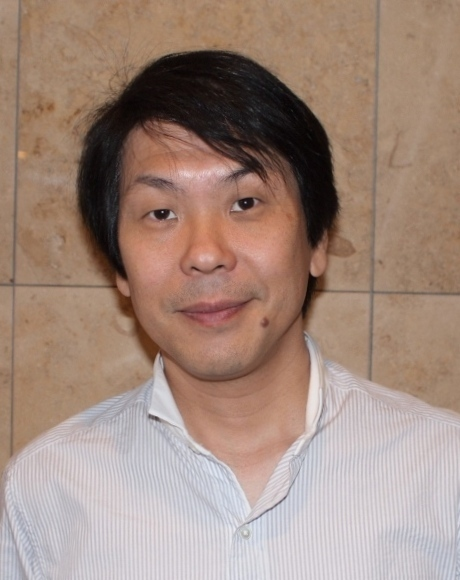
\includegraphics[height=1.5cm]{figs/Inoue-sensei.jpg} \\ \tval{Katsumi INOUE} \\ Professor \& team leader
  \end{tabular}}\right\}\text{\tval{Inoue Laboratory}}$
  &
  $\left.\text{\begin{tabular}{c}
    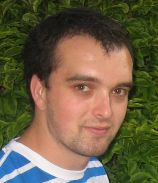
\includegraphics[height=1.5cm]{figs/Loic.jpg} \\ \tval{Loïc PAULEVÉ} \\ Post-doc
  \end{tabular}}\right\}\text{\tval{AMIB}}$
  \\ & \\ & \\
  \multicolumn{2}{l}{$\left.\text{\begin{tabular}{ccc}
      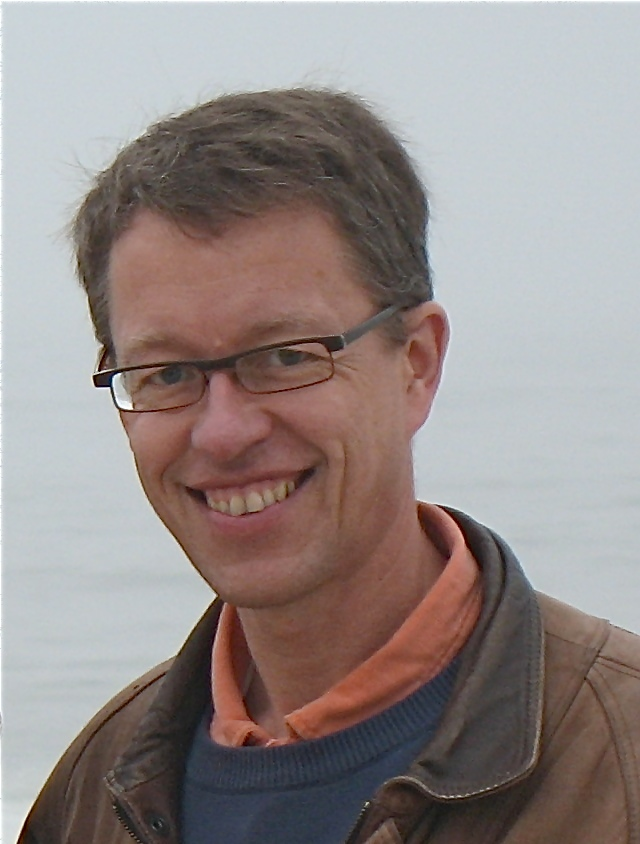
\includegraphics[height=1.5cm]{figs/Olivier.jpg}
    & 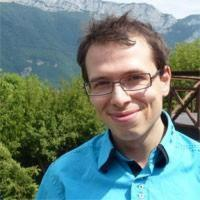
\includegraphics[height=1.5cm]{figs/Morgan.jpg}
    & 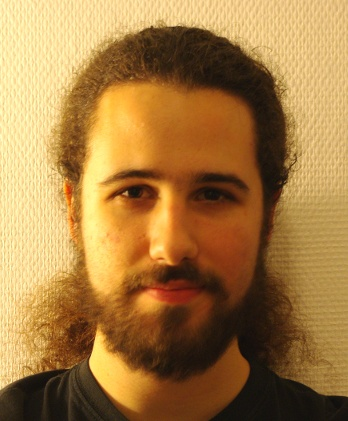
\includegraphics[height=1.5cm]{figs/Moi.jpg} \\
      \tval{Olivier ROUX} & \tval{Morgan MAGNIN} & \tval{Maxime FOLSCHETTE} \\
      Professor \& team leader & Associate professor & $\simeq$ 2\textsuperscript{nd} year PhD student
  \end{tabular}}\right\}\text{\tval{MeForBio}}$}
\end{tabular}
\end{frame}

\appendix
\section[x]{Bibliography}
% Bibliographie

\begin{frame}[c]
  \frametitle{Bibliography}

\footnotesize
\setlength{\parindent}{-1em}
\setlength{\parskip}{0.5em}
~

\vfill
\tcite{Paulevé11} Loïc Paulevé. PhD thesis: \textit{Modélisation, Simulation et Vérification des Grands Réseaux de Régulation Biologique}, October 2011, Nantes, France

%\tcite{PMR10-TSE} Loïc Paulevé, Morgan Magnin, and Olivier Roux. \textit{Tuning Temporal Features within the Stochastic $\pi$-Calculus}. IEEE Transactions on Software Engineering, 37(6):858-871, 2011.

\tcite{PRM10-TCSB} Loïc Paulevé, Morgan Magnin, and Olivier Roux. \textit{Refining dynamics of gene regulatory networks in a stochastic $\pi$-calculus framework}. In Corrado Priami, Ralph-Johan Back, Ion Petre, and Erik de Vink, editors: Transactions on Computational Systems Biology XIII, volume 6575 of Lecture Notes in Computer Science, 171-191. Springer Berlin/Heidelberg, 2011.

\tcite{PMR12-MSCS} Loïc Paulevé, Morgan Magnin, and Olivier Roux. \textit{Static analysis of biological regulatory networks dynamics using abstract interpretation}. Mathematical Structures in Computer Science, in press, 2012.

%\tcite{PR10-CRAS} Loïc Paulevé and Adrien Richard. \textit{Topological Fixed Points in Boolean Networks}. Comptes Rendus de l'Académie des Sciences - Series I - Mathematics, 348(15-16):825 - 828, 2010.

\tcite{RCB08} Adrien Richard, Jean-Paul Comet, and Gilles Bernot. \textit{R. Thomas' logical method}, 2008. Invited at Tutorials on modelling methods and tools: Modelling a genetic switch and Metabolic Networks, Spring School on Modelling Complex Biological Systems in the Context of Genomics.

%\tcite{CMSB12} Maxime Folschette, Loïc Paulevé, Katsumi Inoue, Morgan Magnin, and Olivier Roux. \textit{Concretizing the Process Hitting into Biological Regulatory Networks}. In: Computational Methods in Systems Biology, Springer, 2012.

\vfill
\Large
\begin{flushright}
  \tval{Thank you}\hspace{1cm}~
\end{flushright}
\vfill

~

\end{frame}


\end{document}
